\documentclass[aspectratio=169,
				xcolor=table]{beamer}

% Load general definitions
\usepackage[utf8]{inputenc}
%\usepackage[T1]{fontenc}
\usepackage[brazil]{babel}
\usepackage{amsmath}
\usepackage{amsfonts}
\usepackage{amssymb}
\usepackage{graphicx}
\usepackage{verbatim}
\usepackage{cancel}
\usepackage{askmaps}
\usepackage{tabularx}
\usepackage[table]{xcolor}
%\usepackage{tikz}
\usepackage{multirow}
\usepackage{mathtools}
\usepackage{color, colortbl}
\usepackage{etoolbox}
\usepackage{pbox}
\usepackage{changepage}
\usepackage{xpatch}
\usepackage{array}
\usepackage{marvosym}
\usepackage{tabu}
\usepackage{multicol}
\usepackage{listings}
\usepackage{underscore}
\usepackage{filecontents}
\usepackage[]{algorithm2e}
\usepackage{ragged2e}

\newcolumntype{P}[1]{>{\centering\arraybackslash}m{#1}}
\definecolor{Gray}{gray}{0.75}
\definecolor{Gray2}{gray}{0.85}

\definecolor{lightBlue}{HTML}{DAE8FC}
\definecolor{Blue}{RGB}{51, 51, 204}

%\useinnertheme[lily]{rounded}
\usetheme{UniEvangelica}
%\usetheme{Copenhagen}
%\usetheme{Berlin}
%\usecolortheme{dolphin}
\tolerance=1
\emergencystretch=\maxdimen
\hyphenpenalty=10000
\hbadness=10000

\setbeamertemplate{navigation symbols}{}%remove navigation symbols


\let\olditem=\item% 
\renewcommand{\item}{\olditem \justifying}%
\def\center{\trivlist \centering\item\relax}
\def\endcenter{\endtrivlist}

\setbeamertemplate{itemize/enumerate body begin}{\large}
\setbeamertemplate{itemize/enumerate subbody begin}{\large}

\setbeamertemplate{itemize item}{\raisebox{0.1ex}{$\blacktriangleright$}\hskip0.1em}
\setbeamertemplate{itemize subitem}{\raisebox{0.1ex}{$\blacktriangleright$}\hskip0.1em}

\newcommand{\greenarrow}{\textcolor{green}{\rotatebox[origin=c]{180}{\MVArrowDown}}}

\newcommand{\redarrow}{\textcolor{red}{\MVArrowDown}}

%\newcommand{\ftable}{
%	\begin{table}
%		\large
%		\centering
%		\rowcolors{1}{\ifnumless{\rownum}{2}{Blue}{lightBlue}}{}
%}

\newenvironment{eftable}{
	\begin{table}
		\large
		\centering
		\rowcolors{1}{}{Blue}
		\rowcolors{1}{\ifnumless{\rownum}{2}{Blue}{lightBlue}}{}
	}
	{
	\end{table}
}


%\setbeamertemplate{frametitle}
%{
%	%\vspace*{-2em}	
%	\insertframetitle
%
%	 %\textcolor{white}{\LARGE \insertframetitle}
%
%}

% Specific definitions
\institute[]{\uppercase{Engenharia de Software}}
\title[]{Sistemas Operacionais}
\subtitle[]{Comunicação e Sincronização entre Processos }
\author[]{Prof. M.e Alexandre Tannus}
\date{Anápolis - 2021.1}

%\AtBeginSection{\frame{\tableofcontents[currentsection]}}

\begin{document}
	\begin{frame}
		\titlepage
	\end{frame}

	\begin{frame}
		\tableofcontents
	\end{frame}	
	
	
	\begin{frame}{Questionamentos}
		\begin{itemize}
			\item Como implementar concorrência dentro de uma aplicação?
			\vspace{1em}
			\item E se duas ou mais \textit{threads}/processos quiserem o mesmo recurso?
			\vspace{1em}
			\item Quais regras se aplicam para considerar um sistema concorrente como bem projetado?
		\end{itemize}
	\end{frame}

	\section{Introdução}
	\begin{frame}{Comunicação entre Processos}
		\begin{itemize}
			\item Diferentes processos necessitam se comunicar e podem compartilhar diretamente um espaço de endereçamento
			\vspace{1em}
			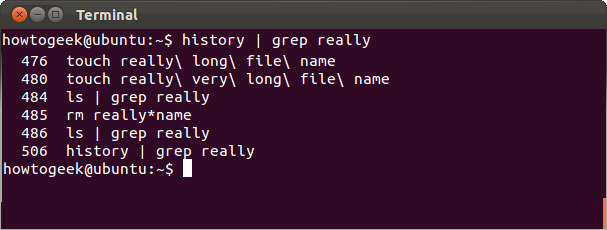
\includegraphics[keepaspectratio, height=0.5\paperheight]{../figs/cap05/history.png} 
		\end{itemize}
	\end{frame}
	
	\begin{frame}{Problemas envolvidos}
		\begin{itemize}
			\item Passagem de informações
			\vspace{1em}
			\item Interferência entre processos em situações críticas
			\vspace{1em}
			\item Sequenciamento adequado entre as dependências
		\end{itemize}
	\end{frame}
	
	\section{Condições de corrida}
	\begin{frame}{Condições de corrida}
		\begin{itemize}			
			\item Situações onde dois os mais processos estão lendo ou escrevendo algum dado compartilhado e o resultado depende de quem processa no momento propício.
		\end{itemize}
			\vspace{1em}
			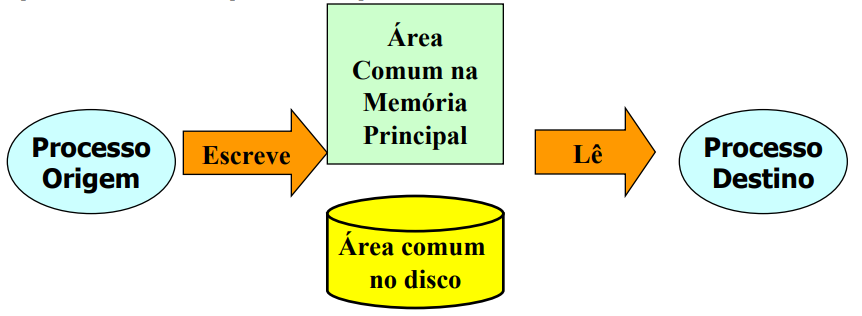
\includegraphics[keepaspectratio, height=0.5\paperheight]{../figs/cap05/race1.png}
	\end{frame}

	
	\begin{frame}{Condições de corrida - Exemplo}
		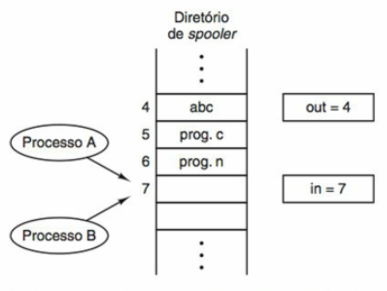
\includegraphics[keepaspectratio, height=0.7\paperheight]{../figs/cap05/race2.png}
	\end{frame}
		
	\begin{frame}{Condições de corrida - Como evitar?}
		\begin{itemize}			
			\item Proibição de ocorrência de múltiplos processos façam uso simultâneo de dados compartilhados (seção crítica).
		\end{itemize}
		
		\vspace{2em}
		
		\huge \centering \alert{EXCLUSÃO MÚTUA}
	\end{frame}
	
	
	\begin{frame}{Condições de corrida - Região crítica}
		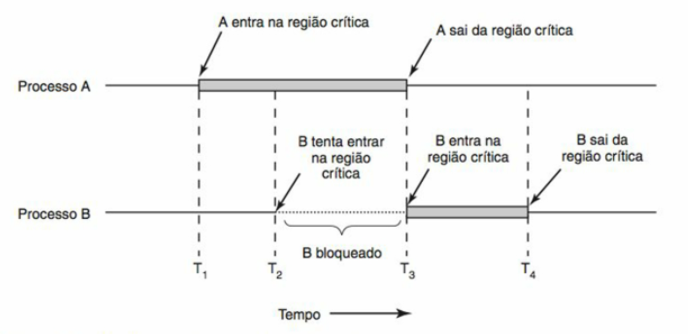
\includegraphics[keepaspectratio, height=0.75\paperheight]{../figs/cap05/regiaocritica.png}
	\end{frame}

	\begin{frame}{Condições para uma boa solução}
		\begin{itemize}
			\item Dois processos não podem estar simultaneamente dentro de uma região crítica.
			\vspace{1em}
			\item Nenhuma suposição pode ser feita sobre as velocidades ou sobre o número de CPUs.
			\vspace{1em}
			\item Nenhum processo executando fora de sua região crítica pode bloquear outros processos.
			\vspace{1em}
			\item Nenhum processo deve ter que esperar eternamente para entrar em sua região crítica. (\textit{starvation}).
		\end{itemize}	
	\end{frame}	
	
	\section{Soluções de Exclusão Mútua}
	\begin{frame}{Soluções para exclusão mútua}
		\begin{itemize}
			\item Espera ocupada
			\vspace{1em}
			\item Primitivas \textit{Sleep/Wakeup}
			\vspace{1em}
			\item Semáforos
			\vspace{1em}
			\item Monitores
			\vspace{1em}
			\item Passagem de mensagem
		\end{itemize}
	\end{frame}
	
	\begin{frame} {Espera Ocupada}
		\begin{itemize}
			\item Constante checagem por algum valor
			\vspace{1em}
			\item Soluções
			\begin{itemize}
				\item Desabilitação de interrupções
				\item Variáveis de travamento (\textit{Lock})
				\item Estrita Alternância
				\item Solução de Peterson
			\end{itemize}
		\end{itemize}
	\end{frame}	
	
	\begin{frame}{Desabilitação das interrupções}
		\begin{itemize}
			\item Solução de \textit{hardware}
			\vspace{1em}
			\item Desabilitação das interrupções quando o processo entra na região crítica e reabilitação quando sai.
			\vspace{1em}
			\item Vantagens
			\begin{itemize}
				\item Simplicidade de implementação
			\end{itemize}
			\vspace{1em}
			\item Desvantagens
			\begin{itemize}
				\item Processo pode esquecer de reabilitar interrupções
				\item Problemas em sistemas \textit{multicore}
			\end{itemize}
		\end{itemize}
	\end{frame}
	
	\begin{frame}{Variáveis de travamento - \textit{Lock}}
		\begin{itemize}
			\item Solução de \textit{software}
			\vspace{1em}
			\item Criação de uma variável \textit{lock}
			\begin{itemize}
				\item Valor 0: Nenhum processo na região crítica
				\item Valor 1: Existe processo na região crítica
			\end{itemize}
		\end{itemize}		
	\end{frame}
	
	\begin{frame}{Variáveis de travamento - \textit{Lock}}
		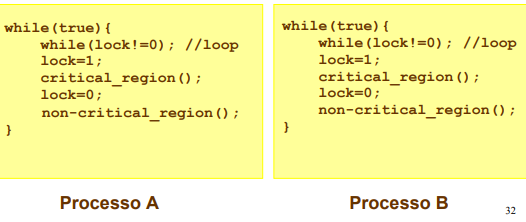
\includegraphics[keepaspectratio, height=0.5\paperheight]{../figs/cap05/lock.png}
	\end{frame}
	
	\begin{frame}{Alternância estrita}
		
		\begin{itemize}
			\item Solução de \textit{software}
			\vspace{1em}
			\item Criação de uma variável \textit{turn}
			\vspace{1em}
			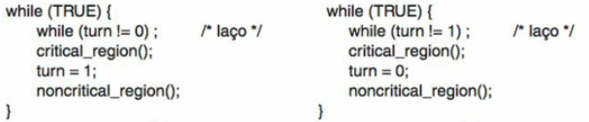
\includegraphics[keepaspectratio, height=0.5\paperheight]{../figs/cap05/turn.png}
		\end{itemize}	
	\end{frame}
	
	\begin{frame}{Solução de Peterson e TSL}
		\begin{itemize}
			\item Solução mista de \textit{hardware/software}
			\vspace{1em}
			\item Variável compartilhada para bloqueio da entrada de um processo na região crítica quando ela estiver ocupada
		\end{itemize}
		
	\end{frame}
	
	\begin{frame}{Espera ocupada - Considerações finais}
		\begin{itemize}
			\item Verificação constante de possibilidade de entrada na região crítica
			\item Desperdício de tempo da CPU
			\item Pode provocar espera infinita (\textit{deadlock}) em determinados sistemas
		\end{itemize}
	\end{frame}
	
	\begin{frame}{Primitivas \textit{Sleep/Wakeup}}
		\begin{itemize}
			\item Bloqueio e desbloqueio de processos
			\begin{itemize}
				\item \textit{Sleep} - Bloqueia o processo (suspensão da execução)
				\item \textit{Wakeup} - Desbloqueio do processo
			\end{itemize}
			\vspace{1em}
			\item Exemplo de uso
			\begin{itemize}
				\item Problema do produtor-consumidor
			\end{itemize}
		\end{itemize}
	\end{frame}
	
	\begin{frame}{Problema do produtor-consumidor}
		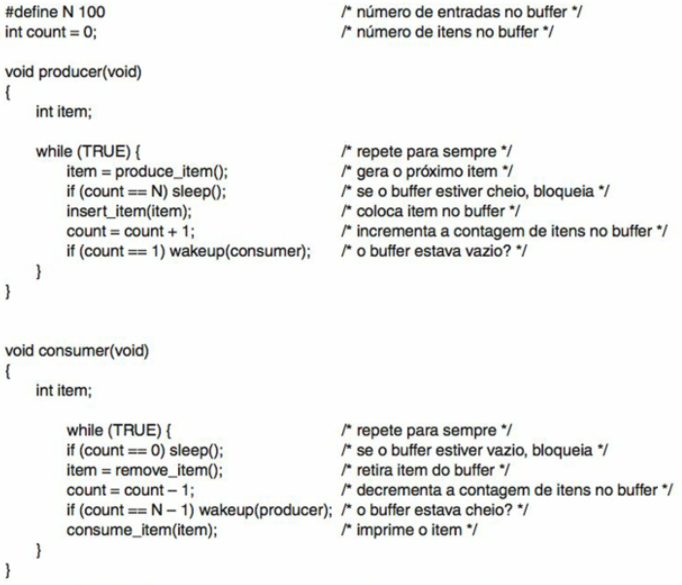
\includegraphics[keepaspectratio, height=0.8\paperheight]{../figs/cap05/produtorconsumidor.png}
	\end{frame}
	
	\begin{frame}{Bibliografia}
		\begin{itemize}
			\item SILBERSCHATZ, A.; GALVIN, P. B.; GAGNE, G.. \textbf{Fundamentos de sistemas operacionais: princípios básicos.} Rio de Janeiro: LTC – Livros Técnicos e Científicos, 2013.
			
			\vspace{1em}

			\item TANENBAUM, A.S., WOODHULL, A.S. \textbf{Sistemas Operacionais.} Porto Alegre: Grupo A, 2008.
			
		\end{itemize}
	\end{frame}


	\begin{frame}{}
	\end{frame}	
	
\end{document}
